\section{Development Model}
\label{sec:development}

To satisfy the mission statement of the Project, the SunPy community adopted an open development model.
This development model is widely used within the scientific Python community.
The \sunpypkg package is hosted on \github and uses \code{git}\footnote{\url{https://git-scm.com/}} as its distributed version control software.
The entire codebase is publicly available and anyone can suggest changes through pull requests.
Since the codebase is licensed under a permissive 2-clause BSD license\footnote{\url{https://opensource.org/licenses/BSD-2-Clause}}, anyone can redistribute, improve, repackage or use it in a closed environment as long as they credit the SunPy developers and redistribute the license.
In order to maintain high quality code, every contribution must satisfy the following requirements:
\begin{enumerate}
    \item Code and documentation must follow widely used style guides (PEP 8 and numpydoc).
    \item All new features must be accompanied with documentation.
    This includes code comments, formal documentation, and gallery examples.
    \item Test code must be provided with coverage reports.
    \item Finally, all code must be within scope and be reviewed and accepted by at least two members of the developer community before it is integrated into the codebase.
\end{enumerate}
These requirements are imposed on every pull request regardless of contributor.

\begin{figure}
    \center
    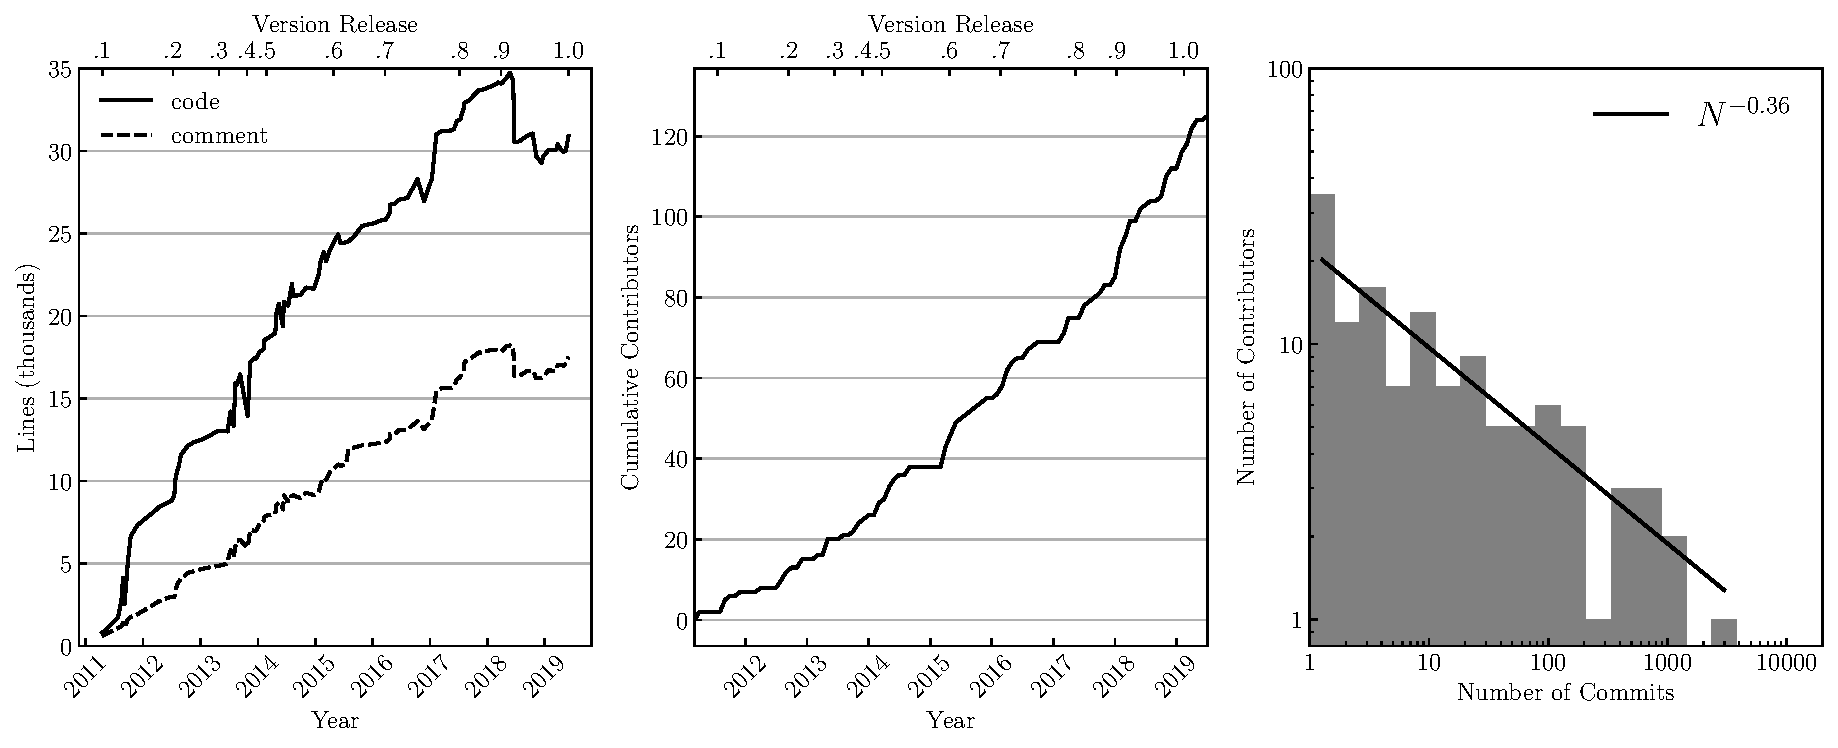
\includegraphics[width = 1.0\textwidth]{figures/dev_meta.pdf}
    \caption{Left panel: A plot of the steady increase in the total number of lines of code (solid line) and documentation line count (dotted line) as a function of time.
	Major releases are indicated.
	A striking reduction in the code base occurred after version 0.9.
	This period saw a major code organization and deletion of obsolete features along with removing support for Python 2.
	Middle panel: The cumulative number of committers (i.e. authors) to \sunpypkg as a function of time shows a steady increase in the number of people involved in the development team.
	Right panel: A plot of the distribution of the number of commits per commiter.
	Though commits is not the best measure this plot does indicates that the majority of commits are undertaken by the least amount of people with an average individual contribution of less than 10 commits.}
\label{fig:metafig}
\end{figure}
